\documentclass[spanish,a4paper,11pt]{article}

\usepackage[dvips]{graphicx}
\usepackage[dvips]{epsfig}
\usepackage[latin1]{inputenc}
\usepackage[spanish]{babel}
\usepackage[T1]{fontenc}

\newcommand{\PI}{{$\pi$ }}
\title{Número $\PI$}
\author{Javier de León Morales}
\date{\today}


\begin{document}
\maketitle
\begin{abstract}
\PI (pi) es la relación entre la longitud de una circunferencia y su diámetro, en geometría euclidiana. Es un número irracional y 
se emplea frecuentemente en matemáticas.
El valor numérico de $\PI$ es:

\begin{equation}
    \PI \approx 3.1415926535897932384626433832
\end{equation}
El valor de π se ha obtenido con diversas aproximaciones a lo largo de la historia. 
La notación con la letra griega \PI proviene de la inicial de las palabras de origen griego περιφέρεια 'periferia' y περίμετρον 'perímetro'.

\end{abstract}

\section{Historia del cálculo del valor de $\PI$}
La búsqueda del mayor número de decimales del número $\PI$ ha supuesto un esfuerzo constante de numerosos científicos a lo largo de la historia. 
Algunas aproximaciones históricas de π son las siguientes.
\subsection{Mesopotamia}
Algunos matemáticos mesopotámicos empleaban, en el cálculo de segmentos, valores de \pi igual a 3, 
alcanzando en algunos casos valores más aproximados, como el de:
\begin{equation}
    \PI \approx 3 + \frac {1}{8} = 3.125
\end{equation}

\subsection{Antigüedad clásica}
Usando un polígono regular inscrito de 384 lados, a finales del siglo V el matemático indio Aryabhata estimó el valor en 3,1416. A mediados del 
siglo VII, estimando incorrecta la aproximación de Aryabhata, Brahmagupta calcula π como \sqrt {10}, cálculo mucho menos preciso que el de su predecesor. 
Hacia 1400 Madhava obtiene una aproximación exacta hasta 11 dígitos (3,14159265359), siendo el primero en emplear series para realizar la estimación.6


\section{Características matemáticas}
Euclides fue el primero en demostrar que la relación entre una circunferencia y su diámetro es una cantidad constante. \PI es:
\begin{itemize}
\item El área de un círculo unitario (de radio unidad del plano euclídeo).
\item El menor número real x positivo tal que \sin(x) = 0.
\end{itemize}
\begin{figure}[!th]
\begin{center}
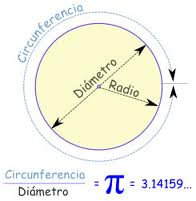
\includegraphics[width=0.25\textwidth]{images/diametro.jpeg}
\caption{Método de Kochanski}
\label{Kochanski}
\end{center}
\end{figure}

\subsection{Las primeras cincuenta cifras decimales}
Los cincuenta primeros son:
\centerline{$\pi \approx 3,14159265358979323846264338327950288419716939937510 $}
En ciencia ciencia e ingeniería, esta constante puede emplearse, la mayoría de las veces, 
con una precisión de sólo una docena de decimales. Con cincuenta decimales se podría describir con precisión la curvatura del Universo con un error más pequeño 
que el tamaño de un protón.

\subsection{Época moderna}
Desde el diseño de la primera computadora se empezaron a desarrollar programas para el cálculo del número \PI con la mayor cantidad de cifras
posible. De esta forma, en 1949 un ENIAC fue capaz de romper todos los récords, obteniendo 2037 cifras decimales en 70 horas. Poco a poco fueron
surgiendo ordenadores que batían récords y, de esta forma, pocos años después (1954) un NORAC llegó a 3092 cifras. Durante casi toda la década
de los años 1960 los IBM fueron batiendo récords, hasta que un IBM 7030 pudo llegar en 1966 a 250.000 cifras decimales (en 8 h y 23 min).
Durante esta época se probaban las nuevas computadoras con algoritmos \footnote{conjunto prescrito de instrucciones o reglas bien definidas, ordenadas 
y finitas que permite realizar una actividad mediante pasos sucesivos que no generen dudas a quien deba realizar dicha actividad.} para la generación de series 
de números procedentes de \PI, en la tabla \ref{tiempo},
podemos observar la evolución de las cifras.

\begin{table}[!ht]
\begin{center}
\begin{tabular}{|c|l|l|l|}
\hline
Año & Descubridor & Ordenador utilizado & Nº de cifras \\ \hline
1949 & G.W. Reitwiesner y otros & ENIAC & 2037 \\ \hline
1954 & & NORAC & 3092 \\ \hline
1959 & Guilloud & IBM 704 & 16167 \\ \hline
1967 & CDC & 6600 & 500000 \\ \hline
1973 & Guillord y Bouyer & CDC 7600 & 1001250 \\ \hline
1981 & Miyoshi y Kanada & FACOM M-200 & 2000036 \\ \hline
1982 & Guilloud & &	2000050 \\ \hline
\end{tabular}
\end{center}
\caption{Evolución del número de cifras}
\label{tiempo}
\end{table}





\bibliographystyle{plain}
\bibliography{bib/references}
\end{document}

